\documentclass[12pt, titlepage]{article}

\usepackage{booktabs}
\usepackage{graphicx}
\usepackage{tabularx}
\usepackage{hyperref}
\hypersetup{
    colorlinks,
    citecolor=black,
    filecolor=black,
    linkcolor=blue,
    urlcolor=blue
}
\usepackage[round]{natbib}
\usepackage{float}
\usepackage{amssymb}

\begin{document}

\title{UNO Flip Remix User Guide}
\author{Mingyang Xu\\ Kevin Ishak\\ Zain-Alabedeen Garada\\ Jianhao Wei\\ Team 24}

\date{\today}

\maketitle

\pagenumbering{roman}

\tableofcontents

\listoffigures


\newpage

\pagenumbering{arabic}

\section{Introduction}
\subsection{Purpose}
This document is intended to served as the user guide for UNO Flip game developed by Team 24 from SFWRENG 4G06A/B captstone course. UNO Flip Remix is a digital version of the classic Uno Flip card game, which is known for its fun and competitive gameplay involving flipping between light and dark card decks. This version aims to preserve the original rules of Uno Flip while adding meaningful strategic improvements and accessible gameplay experiences.

\subsection{Scope}
This user guide covers the installation, setup and usage for the user of the game. It details the process of download, multiplayer connection, the rule of the game, and the basic user interface operations.

\section{Installation}
To set up the system, follow these steps:
\begin{enumerate}
    \item Install visual studio
    \item Clone our repo
    \item Make sure you have a stable internet connection
    \item Make sure the player you want to match is connected to the same network (This include WiFi, Wired connection)
    \item Open the game executable file and enjoy the game!
\end{enumerate}

\section{Usage}
\subsection{Login}
\begin{enumerate}
    \item After the game is launched (as shown in \autoref{fig:g1}), click "Start" button on the main screen
    \item In the box prompted (as shown in \autoref{fig:g2}), enter the name you want other players to see.
    \item You will appear online. If someone is also finding an opponent, you will be matched with that player
\end{enumerate}

\begin{figure}[h]
    \centering
    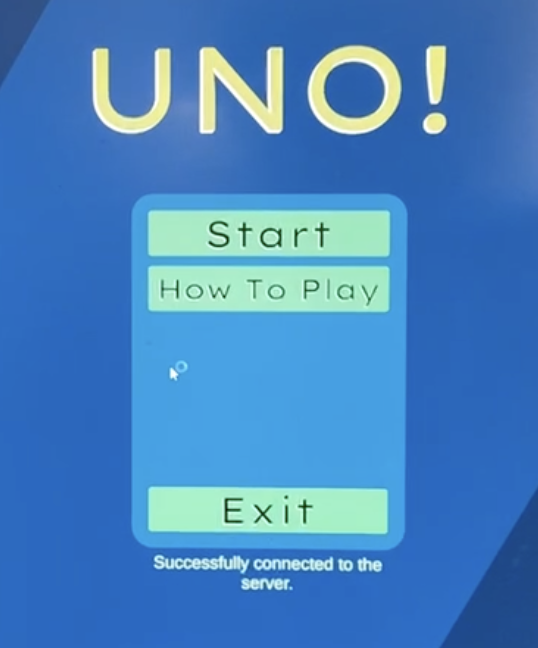
\includegraphics[scale=0.4]{main_Screen.png}
    \caption{Main Screen}
    \label{fig:g1}
\end{figure}

\begin{figure}[h]
    \centering
    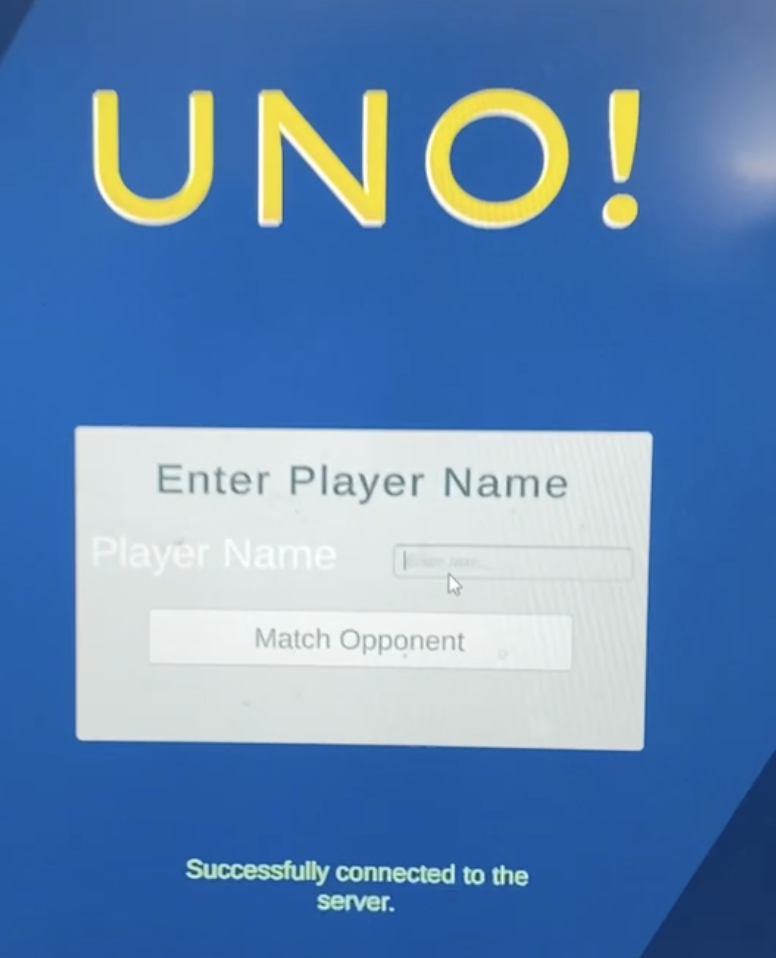
\includegraphics[scale=0.3]{Player_match.png}
    \caption{Player Match Dialogue Box}
    \label{fig:g2}
\end{figure}

\subsection{Match with Other Players}
\begin{enumerate}
    \item After the game is launched, click "Start" button on the main screen (as shown in \autoref{fig:g1}).
    \item In the box prompted, enter the name you want other players to see (as shown in \autoref{fig:g2}).
    \item If there is another player available, there will be a box prompting the name of the other player (as shown in \autoref{fig:g3}). Click "Play Game" to start playing game with that player.
\end{enumerate}

\begin{figure}[h]
    \centering
    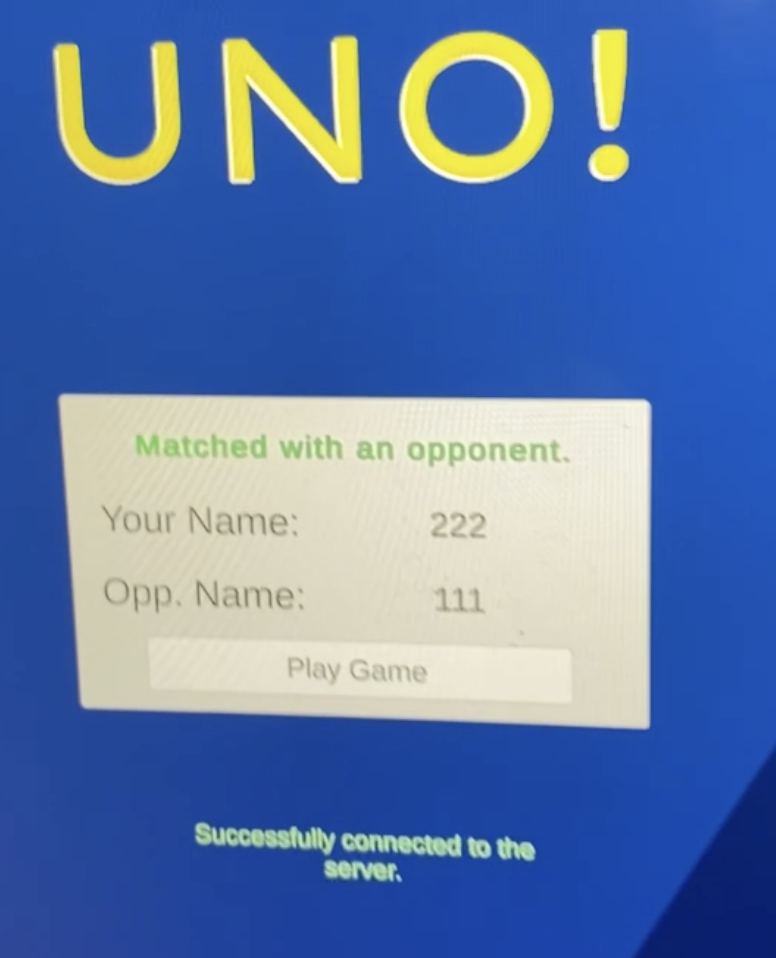
\includegraphics[scale=0.3]{Match_msg.png}
    \caption{Player Match Successful Dialogue Box}
    \label{fig:g3}
\end{figure}


\subsection{Playing the game}
\begin{itemize}
    \item In the game screen (as shown in \autoref{fig:g4}), the cards shown on the lower middle is your card.
    \item There will be two rows: The first row is the dark side of all the cards, the second row is the light side of your cards.
    \item Simply click on the card to play.
    \item The bar on the bottom of the screen shows the turn of current player.
    \item The number beside each card symbol shows how many cards each player has left.
    \item Click on the "UNO" button when you want to tell other people it is the time for UNO. This usually happens when you have one card left.
\end{itemize}

\begin{figure}[h]
    \centering
    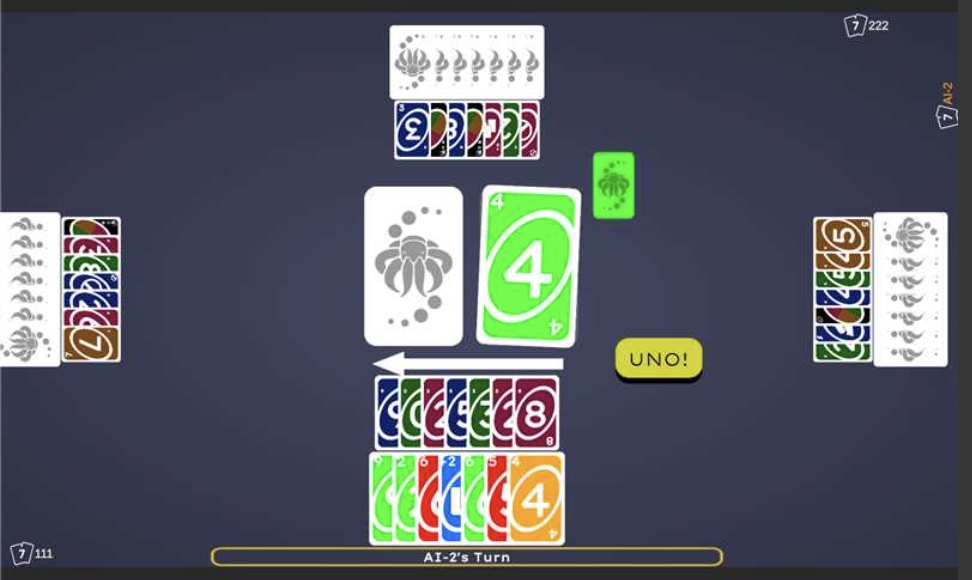
\includegraphics[scale=0.6]{Game_Screen.png}
    \caption{Main Game Screen}
    \label{fig:g4}
\end{figure}


\subsection{End of the game}
\begin{itemize}
    \item When the game end, there will be a dialogue box (as shown in \autoref{fig:g5}) telling you either you win or lost the game.
    \item Click on "Exit" to exit the game, and "Restart" button to restart the game.
\end{itemize}

\begin{figure}[h]
    \centering
    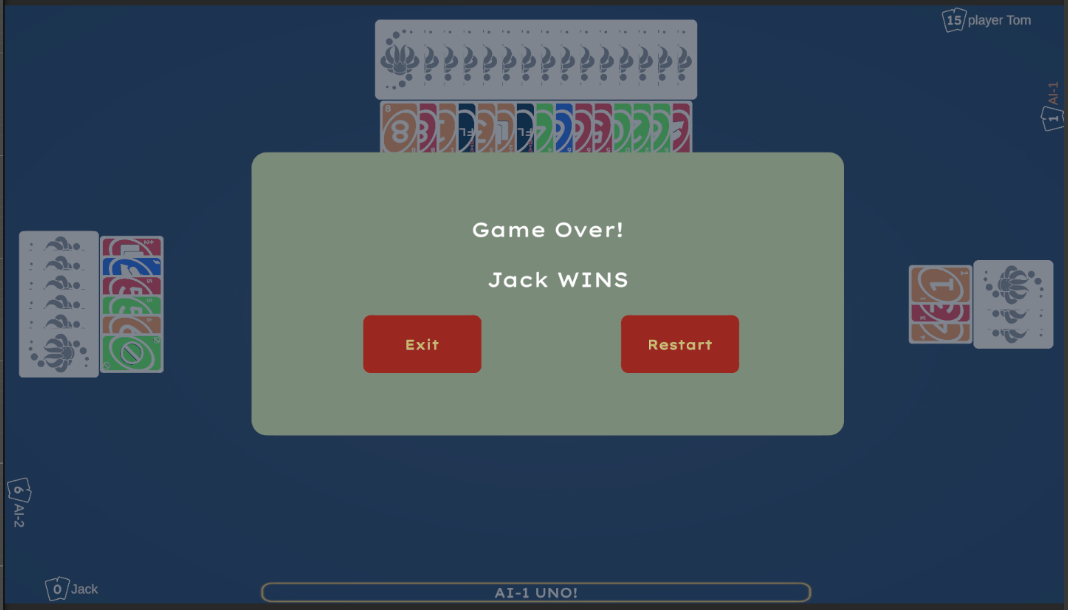
\includegraphics[scale=0.55]{Game_over.png}
    \caption{Main Game Screen}
    \label{fig:g5}
\end{figure}


\end{document}